% !TeX root = ../main.tex
\section{Hệ hỗ trợ quyết định}\label{sec:dss}

Phần OLAP ở mục~\ref{sec:olap} cho nhà quản lý biết chuyện gì đã xảy ra: 6,77\% đơn hàng bị giao trễ, và đơn trễ bị chấm trung bình 2,27 điểm so với 4,29 điểm của đơn đúng hạn. Nhưng biết tỷ lệ trễ của tháng trước không giúp bộ phận vận hành xử lý những đơn đang trên đường. Phần này trình bày thành phần hệ hỗ trợ quyết định (DSS) xây dựng trên kho dữ liệu để trả lời một câu hỏi cụ thể: \textit{khi người bán vừa bàn giao đơn hàng cho đơn vị vận chuyển, đơn nào có nguy cơ giao trễ, và sàn nên chủ động xử lý những đơn nào}.

\subsection{Cách tiếp cận}

DSS của đề tài là một DSS hướng mô hình (model-driven) \cite{turban}, gồm ba thành phần:
\begin{itemize}
    \item \textbf{Dữ liệu:} Data Mart đã xây dựng ở các phần trước.
    \item \textbf{Mô hình:} mô hình Gradient Boosting dự báo xác suất trễ của từng đơn; luật chọn $k$ đơn rủi ro cao nhất khi mỗi ngày chỉ xử lý được $k$ đơn; và mô hình chi phí kỳ vọng kèm phân tích what-if theo các giả định chi phí. Các mô hình được huấn luyện lại mỗi tháng.
    \item \textbf{Giao diện:} trang DSS trên dashboard, nơi người vận hành xem danh sách đơn rủi ro, lý do và hành động đề xuất, rồi duyệt hoặc từ chối từng đề xuất.
\end{itemize}

Quá trình xây dựng DSS đi theo bốn giai đoạn ra quyết định: nhận diện vấn đề (intelligence), thiết kế phương án (design), lựa chọn (choice) và thực hiện (implementation) \cite{turban}. Bảng~\ref{tab:simon} tóm tắt nội dung của từng giai đoạn; các mục tiếp theo đi lần lượt qua từng giai đoạn.

\begin{table}[H]
\centering
\small\setstretch{1.1}
\caption{Bốn giai đoạn ra quyết định áp dụng cho bài toán giao trễ}
\label{tab:simon}
\begin{tabularx}{\linewidth}{|P{2.9cm}|>{\raggedright\arraybackslash}X|P{3.0cm}|}
\hline
\textbf{Giai đoạn} & \textbf{Nội dung trong đề tài} & \textbf{Mục}\\ \hline
Intelligence -- nhận diện vấn đề & Giao trễ làm tỷ lệ đánh giá 1-2 sao tăng từ 9,3\% lên 62,4\%; nguy cơ trễ tăng mạnh khi người bán chuẩn bị hàng lâu và khi đi xa & \ref{sec:edasach}, \ref{sec:olapnghiepvu}, \ref{sec:dssvande}\\ \hline
Design -- thiết kế phương án & Thời điểm can thiệp, các hành động có thể làm, mô hình dự báo xác suất trễ và mô hình chi phí & \ref{sec:dssmohinh}, \ref{sec:dssketqua}\\ \hline
Choice -- lựa chọn & Chọn đơn can thiệp theo năng lực xử lý hoặc theo chi phí kỳ vọng; người dùng chỉnh giả định chi phí (what-if) & \ref{sec:dsschinhsach}\\ \hline
Implementation -- thực hiện & Chấm điểm hằng ngày, ghi kết quả vào schema \code{dss}, người vận hành phê duyệt, huấn luyện lại hằng tháng & \ref{sec:dsstrienkhai}\\ \hline
\end{tabularx}
\end{table}

\subsection{Nhận diện vấn đề và chỉ tiêu}\label{sec:dssvande}

Kết quả khám phá dữ liệu và OLAP cho thấy ba điều. Thứ nhất, giao trễ là nguyên nhân rõ nhất của đánh giá xấu (Hình~\ref{fig:trevadanhgia}). Thứ hai, giao trễ không phân bố đều: có tuyến trễ 1,1\%, có tuyến trễ 23,7\% (Hình~\ref{fig:tuyengiao}); tuần Black Friday trễ gấp ba bình thường (Hình~\ref{fig:blackfriday}). Thứ ba, khi người bán chuẩn bị hàng quá 10 ngày, tỷ lệ trễ lên tới 29,4\% (Hình~\ref{fig:trenhom}). Những điều này cho thấy có thể dự báo trước, ở một mức nào đó, đơn nào dễ trễ.

Thời điểm dự báo được chọn là \textit{lúc người bán bàn giao đơn cho đơn vị vận chuyển}. Lúc này sàn đã biết người bán chuẩn bị hàng nhanh hay chậm, tín hiệu mạnh nhất tìm được ở phần EDA, mà vẫn còn trung vị 21 ngày tới ngày giao dự kiến để làm gì đó: chủ động báo cho khách, tặng voucher hoặc chuyển sang gói vận chuyển nhanh. Mỗi hành động đều có chi phí, và bộ phận vận hành chỉ xử lý được một số đơn mỗi ngày. Quyết định cần hỗ trợ vì vậy là: \textit{mỗi ngày, trong các đơn vừa được bàn giao, chọn những đơn nào để can thiệp}. Hình~\ref{fig:dssflow} là luồng tổng thể của DSS.

% !TeX root = ../../main.tex
% Luồng của thành phần hỗ trợ quyết định: cảnh báo giao trễ lúc bàn giao vận chuyển
\begin{figure}[H]
\centering
\resizebox{\linewidth}{!}{%
\begin{tikzpicture}[
    b/.style={dwbox=#1, text width=2.55cm, minimum height=1.35cm, font=\scriptsize}]
\node[dwdb=dwBlue, minimum width=2.4cm, minimum height=1.6cm, text width=2.2cm, font=\scriptsize] (dm) at (0,0)
  {\textbf{Data Mart}\\\texttt{fact\_sales}\\+ 7 bảng chiều};
\node[b=dwInkTwo, text width=2.75cm, minimum height=2.3cm] (ft) at (3.3,0)
  {\textbf{Đặc trưng point-in-time}\\[1pt] thời gian chuẩn bị hàng, số ngày còn lại, cam kết giao, tuyến, khoảng cách, tỷ lệ trễ gần đây\\[1pt]
   \textcolor{dwMuted}{chỉ dùng thông tin đã biết lúc bàn giao}};
\node[b=dwBlue, text width=2.6cm, minimum height=2.3cm] (m) at (6.85,0)
  {\textbf{Mô hình dự báo}\\[1pt] Gradient Boosting\\+ luật ``đã quá hạn''\\[1pt] $\rightarrow$ P(trễ), mức rủi ro, 3 lý do};
\node[b=dwYellow, text width=2.75cm, minimum height=2.3cm] (pol) at (10.35,0)
  {\textbf{Chính sách quyết định}\\[1pt] theo năng lực: top 5\% (ĐỎ), 5-15\% (VÀNG) mỗi ngày\\[1pt]
   theo chi phí: $p \cdot C_{\text{trễ}} \cdot e > C_{\text{can thiệp}}$};
\node[b=dwBlue, text width=2.3cm, minimum height=2.3cm] (a) at (13.65,0)
  {\textbf{Hành động đề xuất}\\[1pt] báo trước cho khách, voucher, vận chuyển nhanh};
\node[b=dwInkTwo, text width=2.3cm, minimum height=1.1cm] (hu) at (13.65,-3.4) {Người vận hành phê duyệt / từ chối};
\node[dwdb=dwOrange, minimum width=2.6cm, minimum height=1.25cm, text width=2.4cm, font=\scriptsize] (out) at (9.9,-3.4)
  {\textbf{schema \texttt{dss}}\\điểm rủi ro,\\nhật ký quyết định};
\node[b=dwInkTwo, text width=3.0cm, minimum height=1.1cm, draw=dwMuted, dashed] (re) at (3.3,-3.4)
  {\textbf{Huấn luyện lại hằng tháng}\\chỉ dùng đơn đã biết kết quả};
\draw[dwarrow] (dm) -- (ft);
\draw[dwarrow] (ft) -- (m);
\draw[dwarrow] (m) -- (pol);
\draw[dwarrow] (pol) -- (a);
\draw[dwarrow] (a) -- (hu);
\draw[dwarrow] (hu) -- node[dwlabel, above=1pt] {ghi lại} (out);
\draw[dwarrow] (pol.south) -- node[dwlabel, right=1pt] {điểm rủi ro} (pol.south |- out.north);
\draw[dwdash, rounded corners=3pt] (dm.south) |- node[dwlabel, pos=0.3, left=1pt] {kết quả thực tế} (re.west);
\draw[dwdash, rounded corners=3pt] (re.east) -| (m.south);
\end{tikzpicture}}
\caption{Luồng của thành phần hỗ trợ quyết định: dự báo nguy cơ trễ lúc bàn giao vận chuyển, chính sách quyết định và vòng huấn luyện lại}
\label{fig:dssflow}
\end{figure}


Để biết DSS có đủ tốt để dùng hay không, bốn chỉ tiêu định lượng được đặt ra trước khi huấn luyện (Bảng~\ref{tab:chitieu}). Chỉ tiêu chính gắn với năng lực của đội vận hành: giả sử mỗi ngày đội xử lý được khoảng 10\% số đơn bàn giao, thì danh sách 10\% đơn rủi ro nhất phải chứa ít nhất 40\% số đơn sẽ trễ, tức gấp bốn lần chọn ngẫu nhiên. Mức 10\% được chọn vì gần với tỷ lệ trễ thực tế (6,77\%), nên danh sách đủ dài để bao phần lớn đơn trễ mà vẫn vừa sức một đội nhỏ; mục~\ref{sec:dsschinhsach} xét thêm các mức năng lực khác.

\begin{table}[H]
\centering
\small\setstretch{1.1}
\caption{Các chỉ tiêu của mô hình dự báo giao trễ}
\label{tab:chitieu}
\begin{tabularx}{\linewidth}{|P{1.1cm}|>{\raggedright\arraybackslash}X|P{3.4cm}|}
\hline
\textbf{STT} & \textbf{Chỉ tiêu} & \textbf{Ngưỡng}\\ \hline
1 & Tỷ lệ đơn trễ bắt được khi cảnh báo 10\% đơn rủi ro nhất, trung bình tập test & $\geq 40\%$\\ \hline
2 & Khả năng phân biệt đơn trễ và đơn đúng hạn (ROC-AUC) trên tập test & $\geq 0{,}70$\\ \hline
3 & Độ ổn định: tỷ lệ đơn trễ bắt được ở mức 10\% trong từng tháng test & $\geq 30\%$ mọi tháng\\ \hline
4 & Mức rủi ro có ý nghĩa: tỷ lệ trễ thực tế của đơn mức ĐỎ so với đơn mức XANH & gấp ít nhất 5 lần\\ \hline
\end{tabularx}
\end{table}

\subsection{Dữ liệu và đặc trưng}\label{sec:dssmohinh}

\subsubsection{Nhãn và dữ liệu huấn luyện}

Nhãn của bài toán là cờ \code{is\_late} trong bảng fact. Tập huấn luyện được dựng theo hai quy tắc, để mô hình không dùng thông tin mà sàn chưa có tại lúc dự báo.

Quy tắc thứ nhất xử lý các đơn chưa giao. Tại thời điểm dữ liệu dừng (17/10/2018), 1.694 đơn chưa đến tay khách dù đã quá ngày giao dự kiến. Cờ \code{is\_late} của các đơn này để trống vì chưa có ngày nhận hàng, nhưng thực tế chúng chắc chắn trễ, nên được gán nhãn trễ; nếu bỏ đi, các tháng cuối sẽ trông như ít trễ hơn thực tế. Sau bước này có 97.897 đơn có nhãn, tỷ lệ trễ 8,40\%.

Quy tắc thứ hai xác định lúc nào một nhãn được dùng. Ở tháng $M$, sàn chỉ biết một đơn cũ có trễ hay không khi ngày giao dự kiến của đơn đó đã qua: hoặc đơn đã đến tay khách trước hạn, hoặc đã quá hạn mà chưa đến. Vì vậy tập huấn luyện của tháng $M$ chỉ gồm các đơn có ngày giao dự kiến trước ngày đầu tháng $M$. Nếu chỉ lọc theo ngày nhận hàng, trong các đơn gần đây thì đơn giao sớm đã có nhãn còn đơn trễ thì chưa, và mô hình sẽ học sai rằng đơn gần đây thường đúng hạn.

\subsubsection{Đặc trưng}

Mọi đặc trưng được tính từ Data Mart và chỉ dùng thông tin đã biết tại lúc bàn giao (point-in-time). Các tỷ lệ lịch sử của người bán, tuyến hay bang chỉ tính từ những đơn mà kết quả đã biết trước ngày đặt của đơn đang xét, và được làm mượt về tỷ lệ chung khi có ít đơn \cite{han}. Bảng~\ref{tab:dactrungdss} liệt kê các nhóm đặc trưng.

\begingroup\small\setstretch{1.1}
\begin{longtable}{|P{3.3cm}|>{\raggedright\arraybackslash}p{10.4cm}|}
\caption{Các nhóm đặc trưng của mô hình dự báo giao trễ}\label{tab:dactrungdss}\\
\hline
\textbf{Nhóm} & \textbf{Đặc trưng}\\ \hline \endfirsthead
\hline
\textbf{Nhóm} & \textbf{Đặc trưng}\\ \hline \endhead
Khâu chuẩn bị hàng & Thời gian chuẩn bị thực tế, chênh lệch so với thời gian chuẩn bị thường lệ của người bán, số ngày còn lại tới hạn khi bàn giao, thứ bàn giao\\ \hline
Cam kết giao hàng & Số ngày hứa giao (ngày dự kiến $-$ ngày mua); số ngày dư so với thời gian giao thường lệ của tuyến\\ \hline
Địa lý & Bang, vùng của khách và người bán; giao liên bang; khoảng cách Haversine giữa hai thành phố\\ \hline
Đơn hàng & Số sản phẩm, số người bán, giá trị, phí vận chuyển, khối lượng, thể tích, ngành hàng chính, thời gian duyệt\\ \hline
Thời điểm & Tháng, thứ trong tuần, số ngày tới Black Friday\\ \hline
Lịch sử & Tỷ lệ trễ từ trước tới nay của người bán, tuyến, bang khách; số đơn trước đó của người bán và tuyến\\ \hline
Diễn biến gần đây & Tỷ lệ trễ toàn sàn 7 và 30 ngày qua; tỷ lệ trễ 90 ngày của tuyến và người bán; tải đơn của sàn và người bán trong 7 ngày\\ \hline
Đơn tồn đọng & Trong các đơn đã bàn giao 45 ngày qua, tỷ lệ đơn đã quá hạn mà vẫn chưa giao, tính tại ngày bàn giao cho toàn sàn, theo bang khách và theo tuyến\\ \hline
\end{longtable}
\endgroup

Nhóm đặc trưng ``diễn biến gần đây'' cần thiết vì tỷ lệ trễ của các đơn bàn giao biến động rất mạnh giữa các tháng: 14,7\% ở tháng 02/2018, 20,3\% ở tháng 03/2018 nhưng chỉ 1,8\% ở tháng 06/2018 (Hình~\ref{fig:dsstheothang}a). Tỷ lệ lịch sử từ trước tới nay làm mờ đi những đợt biến động này, còn tỷ lệ trễ của 7-30 ngày gần nhất phản ánh ngay khi cả sàn đang gặp sự cố vận chuyển. Ngày nhận hàng, trạng thái đơn, điểm đánh giá và thời gian vận chuyển đều xảy ra sau lúc bàn giao nên bị loại khỏi danh sách đặc trưng; chương trình kiểm tra điều này bằng một câu lệnh \code{assert} ngay khi khởi tạo.

\subsubsection{Cách chia tập và đánh giá}

Dữ liệu có thứ tự thời gian và thay đổi tính chất theo thời gian, nên không thể chia ngẫu nhiên. Cùng một mô hình đơn giản đạt ROC-AUC 0,80 khi chia ngẫu nhiên 80/20 nhưng chỉ 0,59 khi chia theo thời gian, vì khi chia ngẫu nhiên mô hình được học cả từ những tháng nằm sau đơn cần dự báo, điều không thể có trong thực tế.

Mô hình được đánh giá theo kiểu \textit{walk-forward}: với mỗi tháng từ 07/2017 đến 08/2018, mô hình được huấn luyện lại trên dữ liệu đã biết trước tháng đó rồi dự báo cho các đơn của tháng. Năm tháng 01-05/2018 dùng để chọn tham số; ba tháng 06-08/2018, tương ứng khoảng 20\% số đơn cuối cùng, chỉ dùng một lần để báo cáo kết quả. Ba tháng test có 18.753 đơn được bàn giao, trong đó 822 đơn trễ (4,38\%). Với tỷ lệ thấp như vậy, độ chính xác (accuracy) không phải thước đo tốt: đoán ``không trễ'' cho mọi đơn đã đúng 95,6\%. Thước đo chính vì vậy là \textit{tỷ lệ đơn trễ bắt được khi cảnh báo 10\% đơn rủi ro nhất} (một cách chọn ngẫu nhiên sẽ bắt được 10\%), kèm ROC-AUC, PR-AUC và precision, recall, F1 tại các ngưỡng cảnh báo.

\subsection{Kết quả mô hình}\label{sec:dssketqua}

Các phương án được so sánh gồm hai luật đơn giản, Logistic Regression và Gradient Boosting (\code{HistGradientBoostingClassifier} của scikit-learn) \cite{han}. Hai luật là xếp hạng theo tỷ lệ trễ lịch sử của tuyến, và xếp hạng theo số ngày còn lại tới hạn khi bàn giao. Với Gradient Boosting, trước hết một lưới tám bộ tham số được thử trên các tháng validation; bộ tốt nhất của lưới này có \code{learning\_rate} = 0,03, \code{max\_leaf\_nodes} = 15 (số nút lá tối đa của một cây) và \code{min\_samples\_leaf} = 200 (số đơn tối thiểu trong một nút lá, giúp hạn chế overfitting). Để kiểm tra xem còn cải thiện được không, một đợt tìm kiếm mở rộng (TK mở rộng) được chạy thêm, cũng chỉ trên các tháng validation: 60 bộ tham số Gradient Boosting cho mỗi bộ đặc trưng, bốn mức điều chuẩn cho Logistic Regression, ba đặc trưng mới về đơn tồn đọng (tỷ lệ đơn đã bàn giao trong 45 ngày qua đã quá hạn mà chưa giao, tính cho toàn sàn, theo bang khách và theo tuyến), và một mô hình kết hợp ba mô hình tốt nhất bằng trung bình thứ hạng. Hình~\ref{fig:dsssosanh} và Bảng~\ref{tab:dssketqua} so sánh các phương án trên tập test.

\begin{figure}[H]
\centering
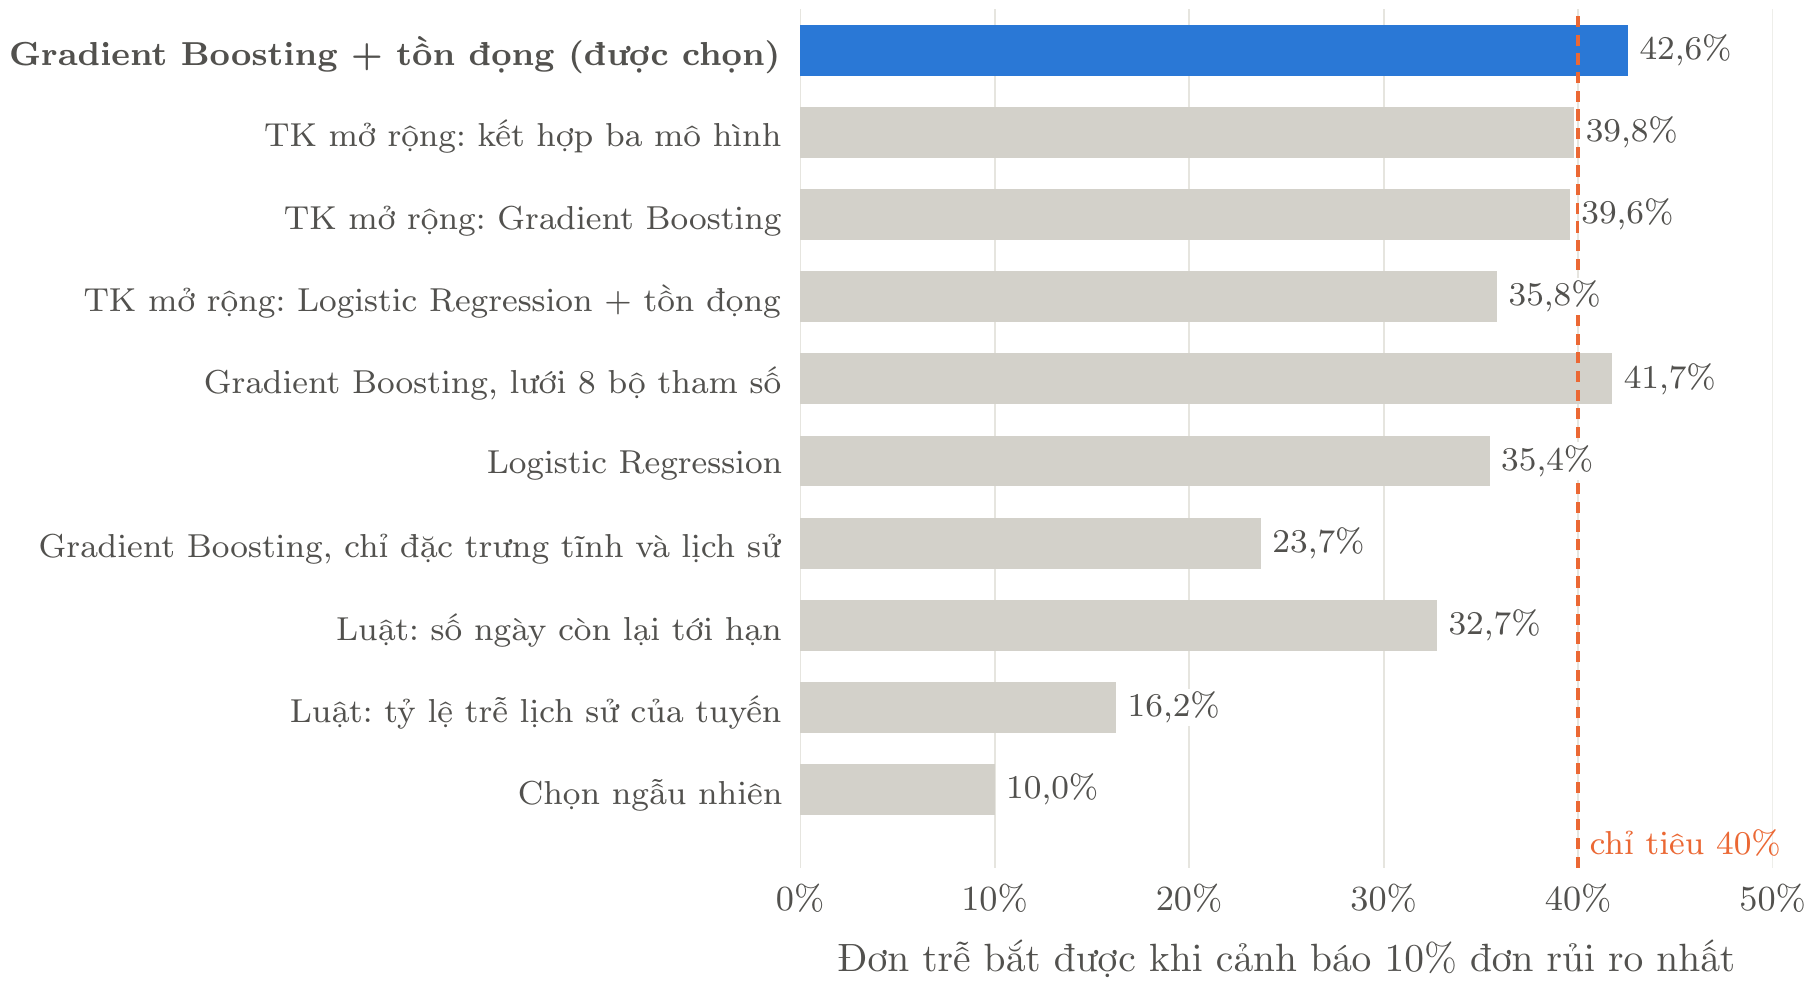
\includegraphics{Pictures/fig-dss-so-sanh-mo-hinh.png}
\caption{Tỷ lệ đơn trễ bắt được khi cảnh báo 10\% đơn rủi ro nhất của các phương án trên tập test 06-08/2018; màu xanh là phương án được chọn}
\label{fig:dsssosanh}
\end{figure}

\begin{table}[H]
\centering
\small\setstretch{1.1}
\caption{Kết quả các phương án trên tập test 06-08/2018 (trung bình ba tháng, huấn luyện lại mỗi tháng); cột cuối là kết quả trên năm tháng validation}
\label{tab:dssketqua}
\begin{tabularx}{\linewidth}{|>{\raggedright\arraybackslash}X|P{1.5cm}|P{1.5cm}|P{2.0cm}|P{2.0cm}|}
\hline
\textbf{Phương án} & \textbf{ROC-AUC} & \textbf{PR-AUC} & \textbf{Bắt được ở 10\% (test)} & \textbf{Bắt được ở 10\% (validation)}\\ \hline
Luật: tỷ lệ trễ lịch sử của tuyến & 0,557 & 0,049 & 16,2\% & 21,4\%\\ \hline
Luật: số ngày còn lại tới hạn & 0,683 & 0,209 & 32,7\% & 10,9\%\\ \hline
Logistic Regression & 0,750 & 0,160 & 35,4\% & 32,3\%\\ \hline
Gradient Boosting, chỉ đặc trưng tĩnh và lịch sử & 0,657 & 0,077 & 23,7\% & 24,0\%\\ \hline
Gradient Boosting, lưới 8 bộ tham số & 0,736 & 0,242 & 41,7\% & 31,9\%\\ \hline
TK mở rộng: Logistic Regression + tồn đọng & 0,749 & 0,162 & 35,8\% & 33,1\%\\ \hline
TK mở rộng: Gradient Boosting & 0,745 & 0,221 & 39,6\% & 33,6\%\\ \hline
TK mở rộng: kết hợp ba mô hình & 0,756 & 0,209 & 39,8\% & 34,3\%\\ \hline
\textbf{TK mở rộng: Gradient Boosting + tồn đọng (được chọn)} & \textbf{0,744} & \textbf{0,254} & \textbf{42,6\%} & \textbf{33,5\%}\\ \hline
\end{tabularx}
\end{table}

Mô hình được chọn bắt được 42,6\% đơn trễ khi chỉ cảnh báo 10\% đơn, gấp hơn bốn lần chọn ngẫu nhiên, với PR-AUC 0,254, gấp 6,8 lần tỷ lệ trễ nền và cao nhất trong các phương án. Logistic Regression có ROC-AUC cao hơn (0,749-0,750), nghĩa là xếp hạng tổng thể tốt tương đương, nhưng ở phần đầu danh sách, phần mà đội vận hành thực sự xử lý, nó chỉ bắt được 35,4-35,8\% đơn trễ; vì quyết định chỉ dựa vào các đơn rủi ro nhất, Gradient Boosting phù hợp hơn. So với cùng thuật toán khi chỉ dùng đặc trưng tĩnh và lịch sử (23,7\%), mức tăng lớn nhất đến từ các đặc trưng lúc bàn giao (thời gian chuẩn bị hàng, số ngày còn lại tới hạn) và các đặc trưng diễn biến gần đây.

Mô hình được chọn không phải phương án cao nhất trên năm tháng validation: vị trí đó thuộc về mô hình kết hợp ba mô hình (34,3\%), nhưng mô hình này chỉ đạt 39,8\% trên test. Năm tháng validation có hai tháng trễ hàng loạt (02 và 03/2018), còn ba tháng test chỉ có khoảng 800 đơn trễ, nên sai số chuẩn của chỉ số vào khoảng $\pm 1{,}7$ điểm phần trăm; chọn theo riêng một giai đoạn ngắn dễ bị nhiễu chi phối. Vì vậy các ứng viên được so sánh trên toàn bộ 14 tháng walk-forward (Bảng~\ref{tab:dsschon}).

\begin{table}[H]
\centering
\small\setstretch{1.1}
\caption{Tỷ lệ đơn trễ bắt được ở mức 10\% của các ứng viên trên từng giai đoạn walk-forward (trung bình theo tháng)}
\label{tab:dsschon}
\begin{tabularx}{\linewidth}{|>{\raggedright\arraybackslash}X|P{1.75cm}|P{1.45cm}|P{1.75cm}|P{1.6cm}|P{1.55cm}|}
\hline
\textbf{Phương án} & \textbf{Validation (5 tháng)} & \textbf{Test (3 tháng)} & \textbf{Năm 2018 (8 tháng)} & \textbf{Cả 14 tháng} & \textbf{ROC-AUC 14 tháng}\\ \hline
Gradient Boosting, lưới 8 bộ tham số & 31,9\% & 41,7\% & 35,6\% & 32,5\% & 0,720\\ \hline
TK mở rộng: Logistic Regression + tồn đọng & 33,1\% & 35,8\% & 34,1\% & 31,5\% & 0,716\\ \hline
TK mở rộng: Gradient Boosting & 33,6\% & 39,6\% & 35,8\% & 32,2\% & 0,728\\ \hline
TK mở rộng: kết hợp ba mô hình & 34,3\% & 39,8\% & 36,4\% & 32,9\% & 0,732\\ \hline
\textbf{TK mở rộng: Gradient Boosting + tồn đọng} & \textbf{33,5\%} & \textbf{42,6\%} & \textbf{36,9\%} & \textbf{33,1\%} & \textbf{0,721}\\ \hline
\end{tabularx}
\end{table}

Gradient Boosting + tồn đọng có kết quả trung bình cao nhất cả trên 14 tháng (33,1\%) lẫn 8 tháng năm 2018 (36,9\%), và tốt hơn mô hình của lưới 8 bộ tham số ở cả bốn giai đoạn; xét từng tháng, nó thắng 8, hòa 2 và thua 4 tháng. Mô hình kết hợp gần ngang về trung bình (32,9\%) và có ROC-AUC tốt hơn, nhưng phải huấn luyện ba mô hình mỗi tháng và kém hơn trên test, nên mô hình đơn được chọn. Vì phép so sánh này có dùng cả ba tháng test, các con số test của mô hình được chọn có thể lạc quan hơn thực tế một chút. Mức tăng so với lưới 8 bộ tham số chủ yếu đến từ bộ tham số mới (\code{learning\_rate} = 0,08, mỗi lần chia nút chỉ xét ngẫu nhiên 50\% đặc trưng) hơn là từ đặc trưng tồn đọng: khi xáo trộn, đặc trưng tồn đọng toàn sàn chỉ làm PR-AUC giảm 0,13 điểm (đứng thứ 10), còn hai đặc trưng tồn đọng theo bang và theo tuyến gần như không đóng góp.

Hình~\ref{fig:dsstheothang} đặt kết quả từng tháng (b) cạnh tỷ lệ trễ của chính tháng đó (a). Ở ba tháng test, mô hình bắt được 40,5\%, 43,0\% và 44,1\% số đơn trễ, ổn định dù tỷ lệ trễ của các tháng này chênh nhau gấp ba (1,8\% ở 06/2018, 5,5\% ở 08/2018). Mô hình của lưới 8 bộ tham số (đường xanh lá) bám sát mô hình được chọn ở hầu hết các tháng; nó nhỉnh hơn ở 10/2017 và 12/2017 nhưng thấp hơn rõ ở 04/2018 (31,6\% so với 37,2\%). Luật theo tuyến chỉ bắt được 6,6\% ở tháng 08/2018, thấp hơn cả chọn ngẫu nhiên.

Đọc hai panel cùng nhau còn thấy một quy luật: đường của mô hình đi xuống đúng vào những tháng cột tỷ lệ trễ vọt lên. Ở 11/2017 và 12/2017 (mùa Black Friday, trễ 12,7\% và 8,2\%) và ở 03/2018 (trễ 20,3\%), mô hình chỉ bắt được 24-27\%. Trong những tháng này đơn trễ hàng loạt vì sự cố chung của khâu vận chuyển chứ không vì đặc điểm riêng của từng đơn, nên việc xếp hạng các đơn với nhau ít tác dụng hơn. Tháng 07/2017 thấp nhất (15,6\%) vì khi đó mới có 11.638 đơn để huấn luyện. Từ 04/2018, khi tập huấn luyện có gần 60 nghìn đơn, kết quả tăng lên 37-44\% và giữ ở mức đó trong cả ba tháng test.

\begin{figure}[H]
\centering
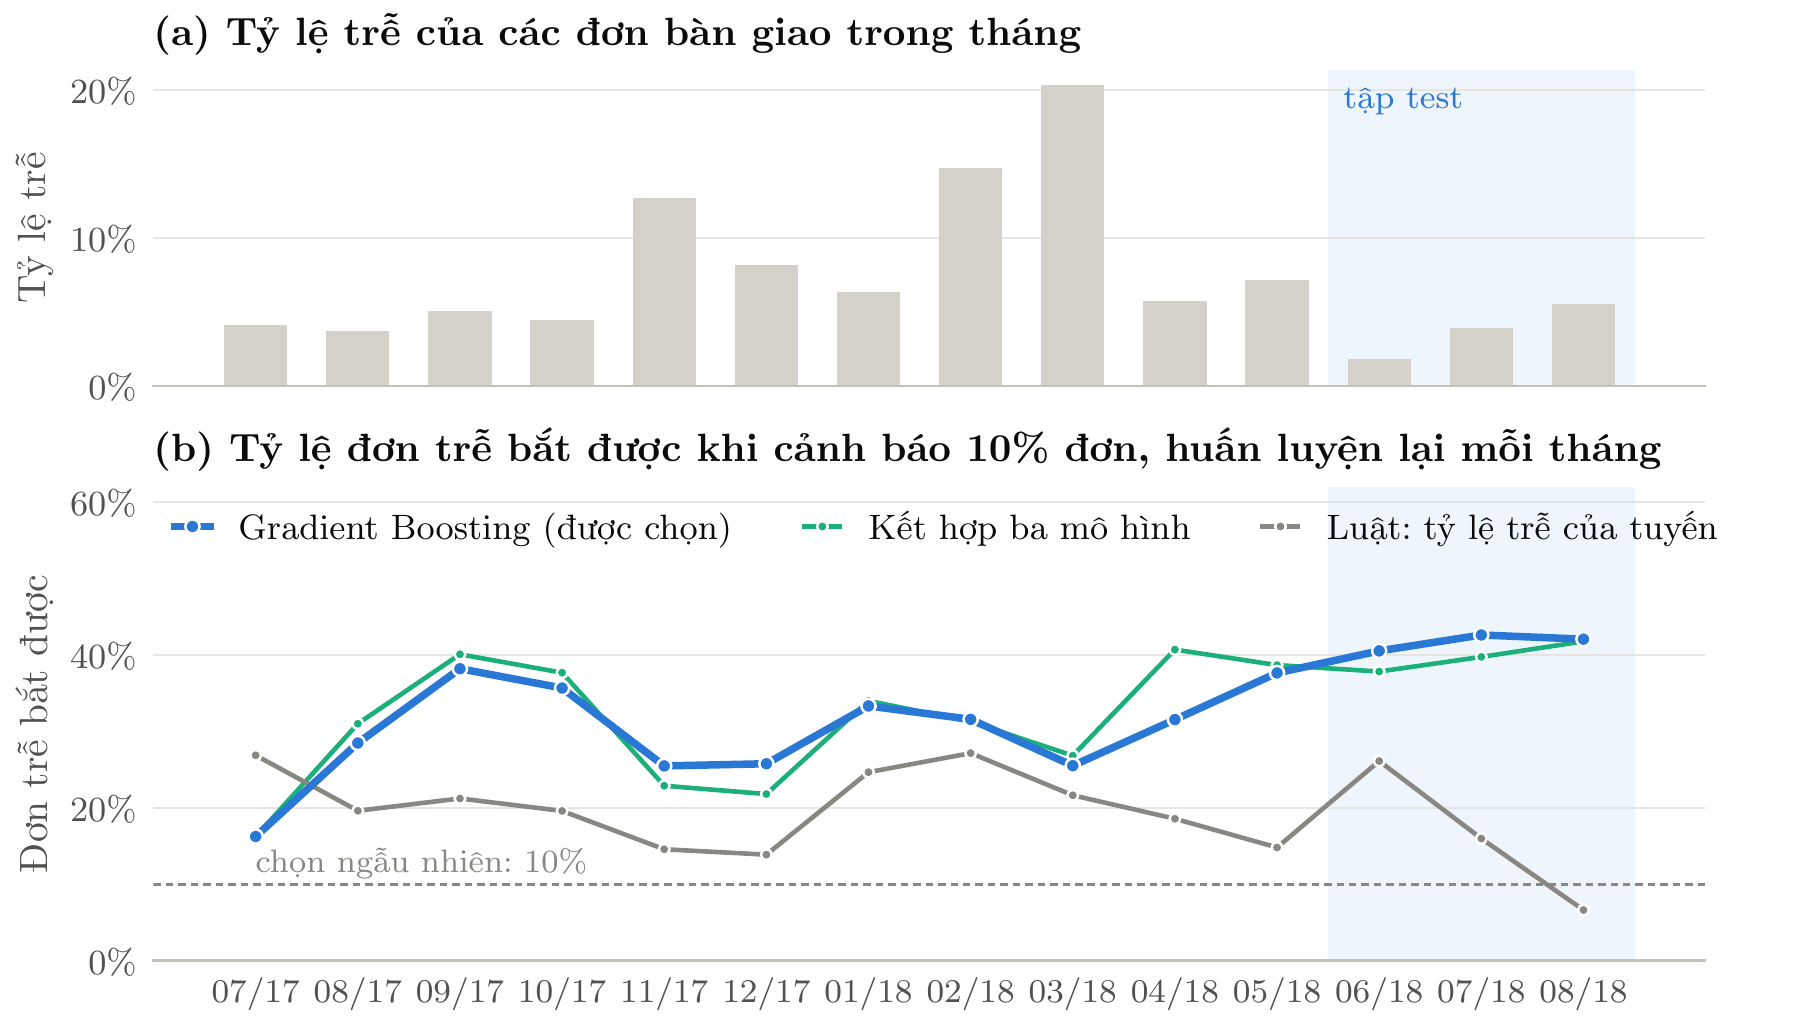
\includegraphics{Pictures/fig-dss-theo-thang.png}
\caption{Tỷ lệ trễ theo tháng (a) và tỷ lệ đơn trễ bắt được khi cảnh báo 10\% đơn, huấn luyện lại mỗi tháng (b); mô hình được chọn là Gradient Boosting (GB) + tồn đọng; vùng tô xanh là tập test}
\label{fig:dsstheothang}
\end{figure}

Bên cạnh mô hình, 120 đơn được bàn giao khi đã quá ngày giao dự kiến (14,6\% số đơn trễ của ba tháng test) được bắt bằng luật mà không cần mô hình, vì các đơn này chắc chắn trễ. Kết hợp mô hình và luật này, DSS bắt được 46,5\% số đơn trễ khi cảnh báo 10\% số đơn bàn giao mỗi ngày.

Để biết mô hình dựa vào đâu, mức giảm PR-AUC được đo khi xáo trộn ngẫu nhiên từng đặc trưng (permutation importance) trên tháng test cuối cùng (Hình~\ref{fig:dssdactrung}). Số ngày còn lại tới hạn khi bàn giao chiếm ưu thế tuyệt đối (PR-AUC giảm 28,8 điểm khi xáo trộn đặc trưng này), cách xa các đặc trưng tiếp theo: thời gian chuẩn bị thực tế (2,0 điểm), người bán chuẩn bị hàng chậm hơn thường lệ của chính họ (1,8 điểm) và độ dư của ngày hứa giao so với thời gian giao thường lệ của tuyến (1,4 điểm). Các đặc trưng còn lại, như tỷ lệ trễ lịch sử của bang khách hay thứ bàn giao, chỉ đóng góp dưới 1 điểm. Kết quả này khớp với phần EDA và với trực giác nghiệp vụ: người bán giữ hàng càng lâu thì đơn vị vận chuyển càng ít thời gian. Đây cũng là cơ sở để sinh các lý do hiển thị cho người vận hành ở mục~\ref{sec:dsstrienkhai}.

\begin{figure}[H]
\centering
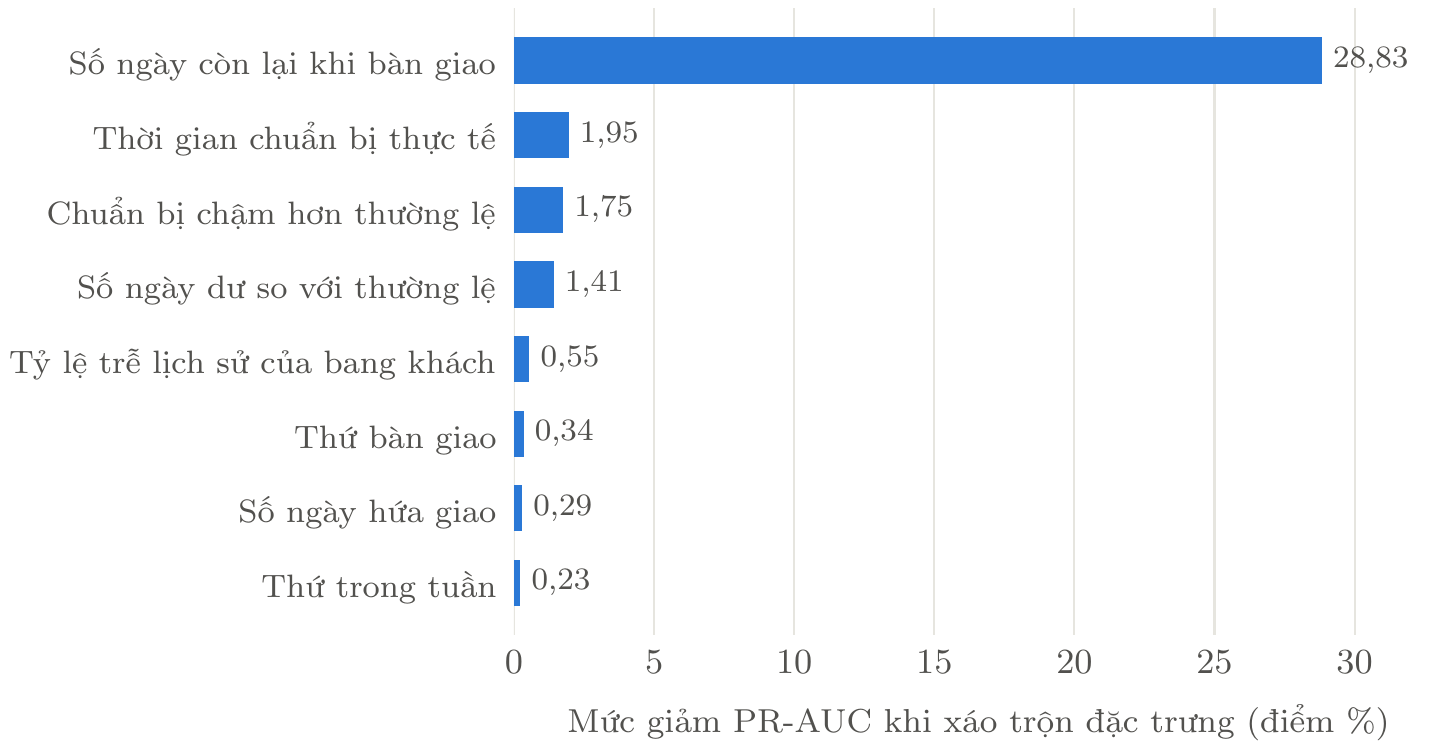
\includegraphics{Pictures/fig-dss-dac-trung.png}
\caption{Tám đặc trưng quan trọng nhất của mô hình (permutation importance, tháng 08/2018)}
\label{fig:dssdactrung}
\end{figure}

Hình~\ref{fig:dssmatran} là ma trận nhầm lẫn của DSS trên ba tháng test ở hai mức cảnh báo được dùng trong thực tế (mục~\ref{sec:dsschinhsach}). Khi chỉ cảnh báo mức ĐỎ, cứ khoảng ba đơn bị cảnh báo thì có một đơn thật sự trễ (precision 30,8\%: 285 đúng, 640 cảnh báo nhầm), và DSS bắt được 34,7\% số đơn trễ; 537 đơn trễ còn lại không bị cảnh báo. Mở rộng sang cả mức VÀNG thì bắt được 54,0\% (444 đơn) nhưng precision giảm còn 16,0\%. Accuracy ở cả hai mức (93,7\% và 85,5\%) đều thấp hơn mức 95,6\% của cách đoán ``không trễ'' cho mọi đơn, một lần nữa cho thấy vì sao không dùng accuracy để đánh giá bài toán này.

\begin{figure}[H]
\centering
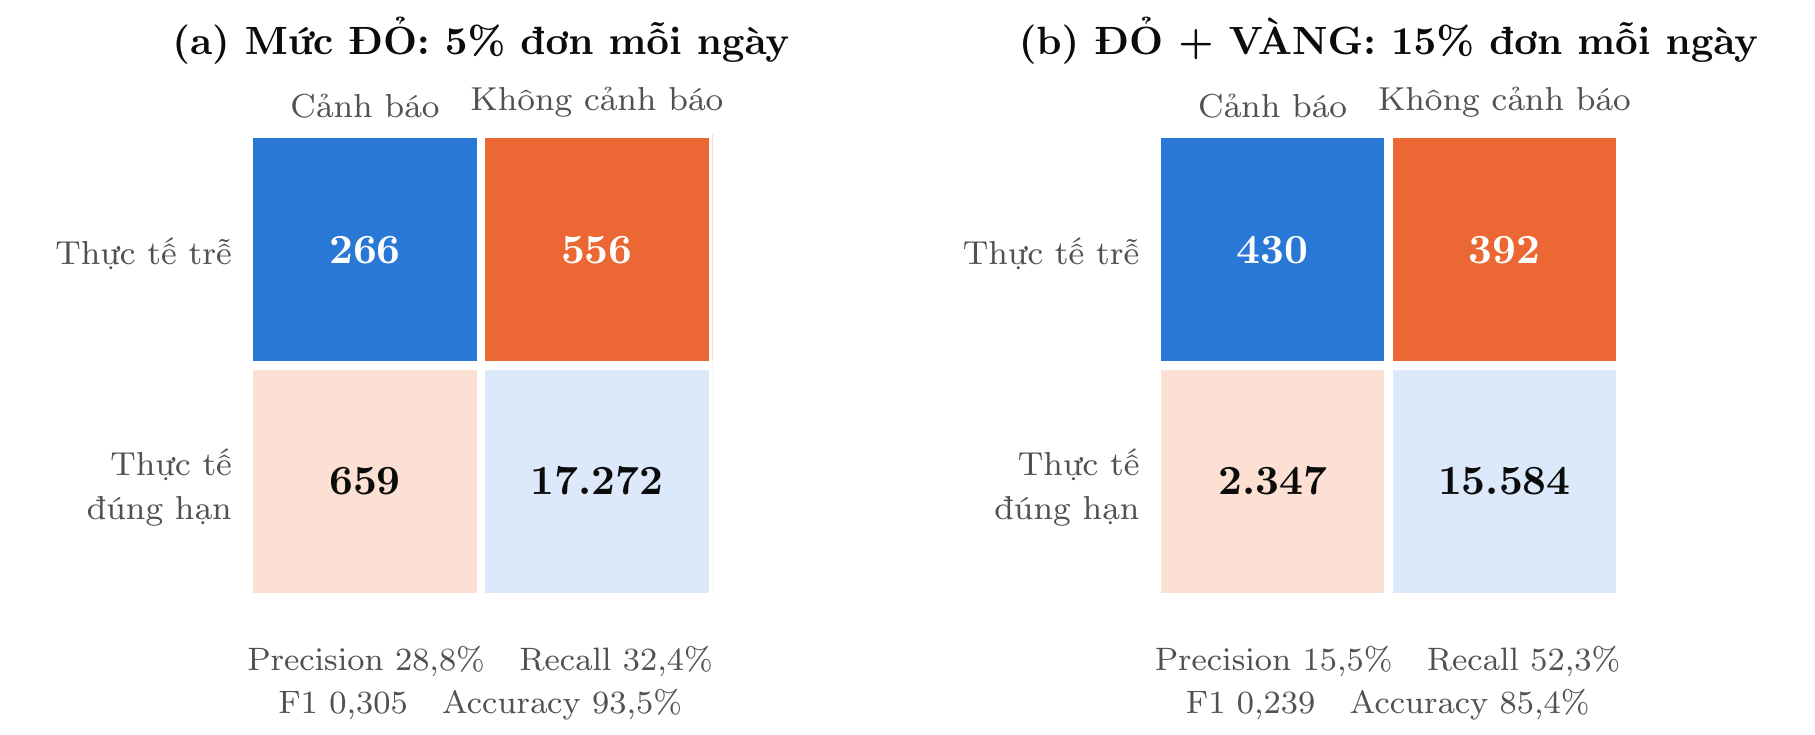
\includegraphics{Pictures/fig-dss-ma-tran-nham-lan.png}
\caption{Ma trận nhầm lẫn của DSS trên 18.753 đơn bàn giao trong ba tháng test, ở hai mức cảnh báo}
\label{fig:dssmatran}
\end{figure}

Bảng~\ref{tab:datchitieu} đối chiếu kết quả với các chỉ tiêu đã đặt ở Bảng~\ref{tab:chitieu}: cả bốn chỉ tiêu đều đạt.

\begin{table}[H]
\centering
\small\setstretch{1.1}
\caption{Đối chiếu kết quả của DSS với các chỉ tiêu}
\label{tab:datchitieu}
\begin{tabularx}{\linewidth}{|>{\raggedright\arraybackslash}X|P{2.4cm}|P{3.6cm}|P{1.4cm}|}
\hline
\textbf{Chỉ tiêu} & \textbf{Ngưỡng} & \textbf{Kết quả} & \textbf{Đánh giá}\\ \hline
Đơn trễ bắt được ở mức 10\% & $\geq 40\%$ & 42,6\% (mô hình); 46,5\% (kèm luật) & Đạt\\ \hline
ROC-AUC trên tập test & $\geq 0{,}70$ & 0,744 & Đạt\\ \hline
Ổn định qua từng tháng test & $\geq 30\%$ mọi tháng & 40,5\%; 43,0\%; 44,1\% & Đạt\\ \hline
Tỷ lệ trễ của mức ĐỎ so với mức XANH & gấp ít nhất 5 lần & 30,8\% so với 2,4\% (13,0 lần) & Đạt\\ \hline
\end{tabularx}
\end{table}

\subsection{Chính sách quyết định}\label{sec:dsschinhsach}

Mô hình chỉ cho ra xác suất trễ. Việc chọn đơn nào để can thiệp là một quyết định trong điều kiện rủi ro: với mỗi đơn ta biết xác suất xảy ra kết quả xấu chứ không biết chắc kết quả \cite{turban}. DSS đưa ra hai chính sách để người quản lý chọn tùy tình huống.

\subsubsection{Chính sách theo năng lực xử lý}

Khi đội vận hành chỉ xử lý được một số đơn cố định mỗi ngày, DSS xếp hạng các đơn bàn giao trong ngày theo điểm rủi ro và gán ba mức: ĐỎ cho 5\% đơn rủi ro nhất, VÀNG cho 10\% tiếp theo, XANH cho phần còn lại; mọi đơn đã quá hạn khi bàn giao đều được xếp ĐỎ. Hình~\ref{fig:dssmucruiro} kiểm chứng cách xếp mức này trên ba tháng test: 30,8\% trong 925 đơn ĐỎ thực sự bị trễ, 8,6\% trong 1.852 đơn VÀNG, còn 15.976 đơn XANH chỉ trễ 2,4\%. Tỷ lệ trễ giảm dần đúng theo thứ tự mức rủi ro, và đơn ĐỎ trễ nhiều gấp 13,0 lần đơn XANH; ba mức vì vậy có ý nghĩa thực tế để phân bổ công sức theo dõi.

\begin{figure}[H]
\centering
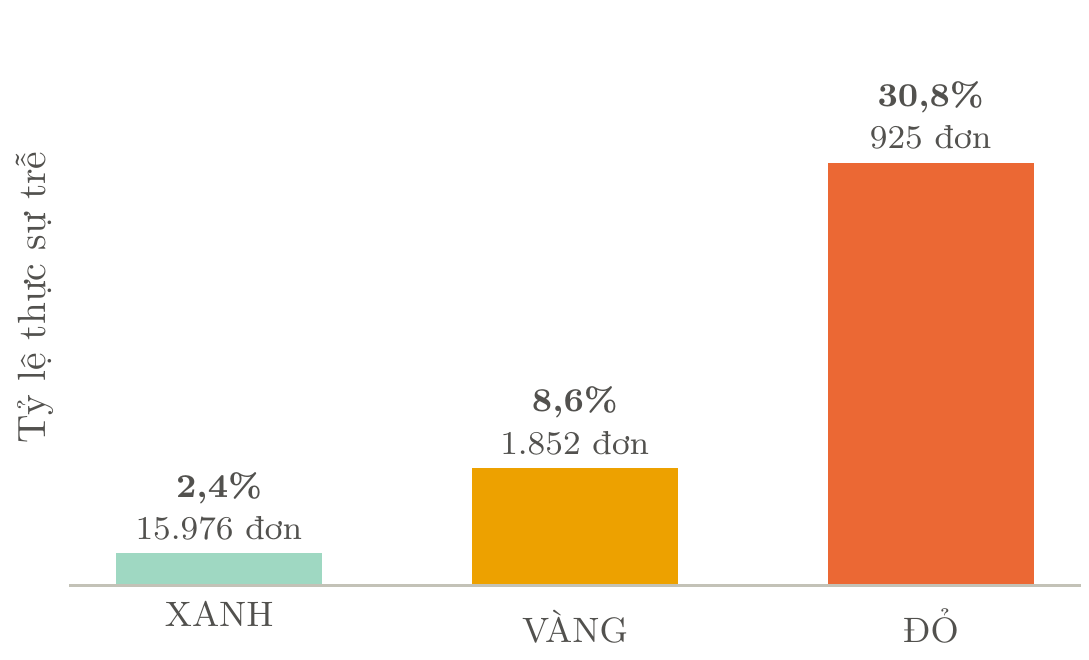
\includegraphics{Pictures/fig-dss-muc-rui-ro.png}
\caption{Tỷ lệ đơn thực sự trễ trong từng mức rủi ro, ba tháng test 06-08/2018}
\label{fig:dssmucruiro}
\end{figure}

Hình~\ref{fig:dssnangluc} cho người quản lý thấy đánh đổi giữa năng lực và hiệu quả: xử lý 5\% đơn mỗi ngày thì bắt được 35\% số đơn trễ, 10\% thì bắt được 47\%, 15\% thì bắt được 54\%, còn 30\% thì bắt được 67\%. Đường cong dốc ở đầu rồi thoải dần, nghĩa là những đơn được xử lý đầu tiên mang lại nhiều giá trị nhất, còn mở rộng năng lực quá 15-20\% thì lợi ích tăng thêm không nhiều.

\begin{figure}[H]
\centering
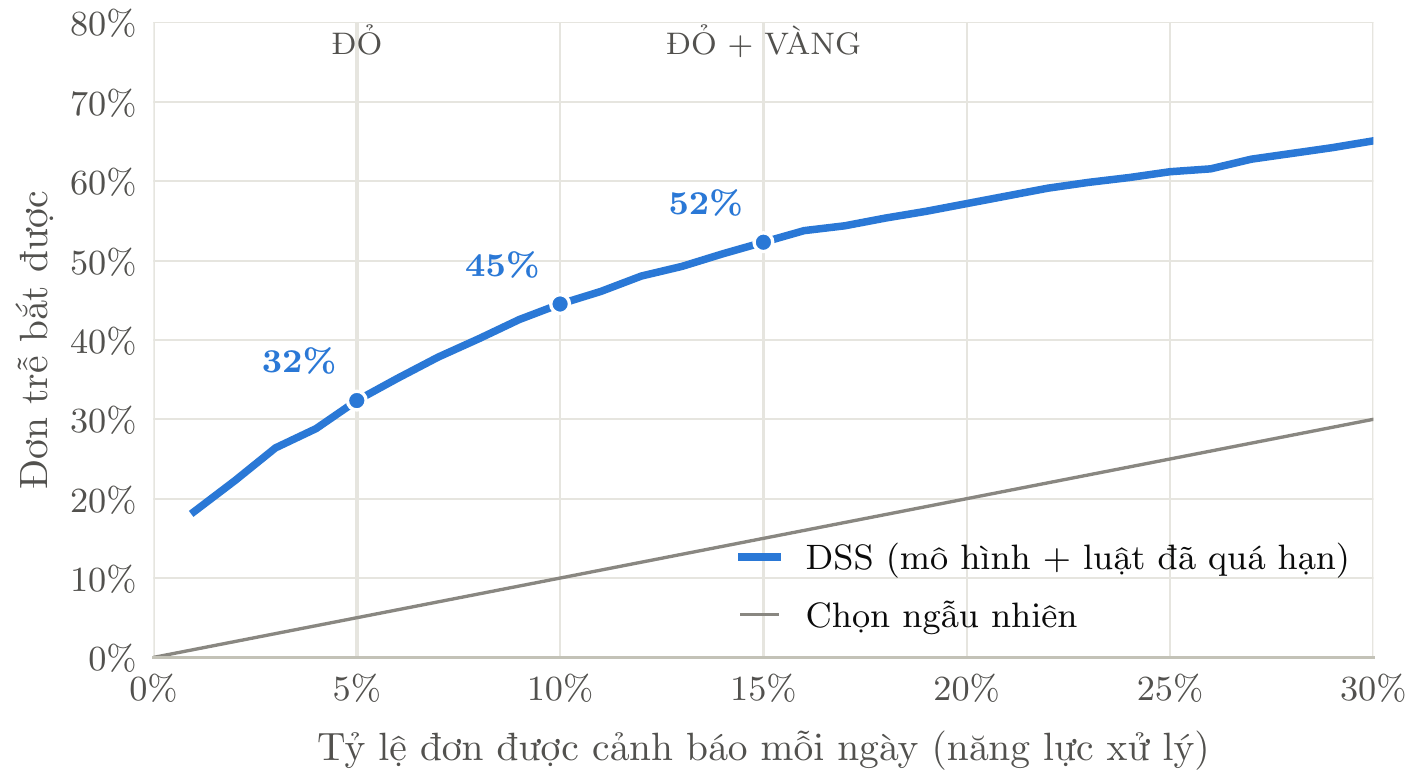
\includegraphics{Pictures/fig-dss-nang-luc.png}
\caption{Tỷ lệ đơn trễ bắt được theo năng lực xử lý mỗi ngày, ba tháng test}
\label{fig:dssnangluc}
\end{figure}

\subsubsection{Chính sách theo chi phí kỳ vọng}

Khi hành động can thiệp tốn tiền, như tặng voucher, nên quyết định theo giá trị kỳ vọng. Gọi $p$ là xác suất trễ (đã hiệu chỉnh bằng isotonic regression trên 60 ngày gần nhất), $C_{\text{trễ}}$ là thiệt hại khi một đơn bị trễ, $e$ là tỷ lệ thiệt hại tránh được nhờ can thiệp và $C_{\text{can thiệp}}$ là chi phí can thiệp một đơn. Can thiệp có lợi khi
\[
p \cdot C_{\text{trễ}} \cdot e > C_{\text{can thiệp}}
\quad\Longleftrightarrow\quad
p > p^{*} = \frac{C_{\text{can thiệp}}}{C_{\text{trễ}} \cdot e}.
\]
Các tham số chi phí không có trong dữ liệu, nên DSS dùng giả định mặc định và cho người dùng chỉnh lại trên dashboard (what-if). Giả định mặc định là $C_{\text{trễ}} = 30$ BRL (khoảng 22\% giá trị đơn trung bình, gồm chi phí hỗ trợ khách và phần giá trị khách hàng có thể mất), hành động là liên hệ khách và tặng voucher với $C_{\text{can thiệp}} = 8$ BRL, $e = 0{,}4$; khi đó $p^{*} = 0{,}667$. Bảng~\ref{tab:dsschinhsach} là kết quả backtest các chính sách trên ba tháng test. Số đánh giá 1-2 sao tránh được được ước tính bằng số đơn trễ bắt được nhân $e$ nhân mức chênh tỷ lệ đánh giá thấp giữa đơn trễ và đơn đúng hạn (62,4\% $-$ 9,3\%).

\begin{table}[H]
\centering
\small\setstretch{1.1}
\caption{Backtest các chính sách quyết định trên ba tháng test (18.753 đơn bàn giao)}
\label{tab:dsschinhsach}
\begin{tabularx}{\linewidth}{|>{\raggedright\arraybackslash}X|P{1.6cm}|P{1.9cm}|P{1.9cm}|P{1.8cm}|P{1.7cm}|}
\hline
\textbf{Chính sách} & \textbf{Số đơn can thiệp} & \textbf{Đơn trễ bắt được} & \textbf{Precision} & \textbf{Lợi ích ròng (BRL)} & \textbf{Đánh giá xấu tránh được}\\ \hline
Mức ĐỎ (5\%) & 925 & 285 (34,7\%) & 30,8\% & $-$3.980 & 61\\ \hline
ĐỎ + VÀNG (15\%) & 2.777 & 444 (54,0\%) & 16,0\% & $-$16.888 & 94\\ \hline
Chi phí kỳ vọng ($p^{*} = 0{,}667$) & 238 & 212 (25,8\%) & 89,1\% & 640 & 45\\ \hline
\end{tabularx}
\end{table}

Bảng~\ref{tab:dsschinhsach} cho thấy điều mà con số dự báo đơn lẻ không nói được. Tặng voucher cho cả 15\% đơn rủi ro nhất lỗ gần 17 nghìn BRL, vì precision 16,0\% chưa đủ bù chi phí; chính sách chi phí kỳ vọng chỉ tặng voucher cho 238 đơn có xác suất trễ cao (precision 89,1\%) và có lãi. Trong 238 đơn này, 120 đơn đến từ luật ``đã quá hạn khi bàn giao'' và 118 đơn do mô hình chọn; 92 trong 118 đơn đó trễ thật (78\%), tức là sau khi hiệu chỉnh, mô hình vẫn tìm thêm được một nhóm đơn rất dễ trễ mà luật không bắt được. Cách hợp lý vì vậy là kết hợp: với các đơn ĐỎ chỉ báo trước cho khách, việc gần như không tốn tiền, còn voucher chỉ dành cho các đơn vượt ngưỡng $p^{*}$. Kết luận này phụ thuộc vào giả định chi phí: chẳng hạn nếu voucher chỉ giữ lại được 20\% thiệt hại ($e = 0{,}2$) thì $p^{*}$ vượt quá 1, DSS chỉ còn đề xuất voucher cho các đơn đã chắc chắn trễ. Vì vậy các tham số này được để mở cho người quản lý chỉnh theo số liệu thực tế của sàn.

\subsection{Triển khai và giao diện}\label{sec:dsstrienkhai}

Ở mỗi kỳ chạy, chương trình \code{score\_delay.py} huấn luyện lại mô hình trên các đơn đã biết kết quả, hiệu chỉnh xác suất, chấm điểm các đơn mới được bàn giao, gán mức rủi ro và ghi vào bảng \code{dss.delay\_risk\_score}; thông tin của từng phiên bản mô hình (dữ liệu huấn luyện, kết quả đánh giá) được lưu ở \code{dss.model\_registry}. Với ba tháng test, bảng điểm có 18.753 dòng ứng với ba phiên bản mô hình.

Để người vận hành hiểu vì sao một đơn bị cảnh báo, mỗi đơn ĐỎ hoặc VÀNG có tối đa ba lý do bằng tiếng Việt. Lý do được sinh từ các đặc trưng quan trọng ở Hình~\ref{fig:dssdactrung}: đặc trưng nào của đơn lệch xa mức bình thường nhất thì được nêu trước. Trong 925 đơn ĐỎ, lý do đứng đầu phổ biến nhất là tỷ lệ trễ cao của tuyến (350 đơn), ngày hứa giao quá sát (181 đơn), người bán chuẩn bị hàng chậm hơn thường lệ (124 đơn), đơn đã quá hạn khi bàn giao (120 đơn) và chỉ còn ít ngày tới hạn (92 đơn). Bảng~\ref{tab:dssvidu} là ba đơn ĐỎ trễ thật và ba đơn ĐỎ vẫn đúng hạn, chọn ngẫu nhiên trong tháng 07/2018. Ba đơn trễ có cùng một kiểu lý do rất rõ: người bán giữ hàng lâu hơn thường lệ 15-21 ngày, khi bàn giao chỉ còn 0-1 ngày tới hạn, và mô hình cho xác suất trễ gần như chắc chắn (1,00). Ba đơn đúng hạn bị cảnh báo chủ yếu vì yếu tố tuyến (tuyến SP$\rightarrow$BA hay trễ, ngày hứa giao sát) hoặc người bán có tỷ lệ trễ gần đây cao, là những yếu tố làm tăng rủi ro nhưng không quyết định; xác suất của chúng chỉ khoảng 0,09-0,19. Người vận hành vì vậy có thể dùng cả mức xác suất lẫn loại lý do để quyết định mức độ can thiệp.

\begingroup\small\setstretch{1.1}
\begin{longtable}{|P{1.6cm}|P{1.0cm}|>{\raggedright\arraybackslash}p{8.2cm}|P{1.6cm}|}
\caption{Ví dụ đầu ra của DSS: ba đơn ĐỎ trễ thật và ba đơn ĐỎ đúng hạn, chọn ngẫu nhiên trong tháng 07/2018}\label{tab:dssvidu}\\
\hline
\textbf{Tuyến} & \textbf{$p$} & \textbf{Lý do hiển thị cho người vận hành} & \textbf{Thực tế}\\ \hline \endfirsthead
\hline
\textbf{Tuyến} & \textbf{$p$} & \textbf{Lý do hiển thị cho người vận hành} & \textbf{Thực tế}\\ \hline \endhead
SP$\rightarrow$MG & 1,00 & Người bán chuẩn bị hàng chậm hơn thường lệ 21 ngày; chỉ còn 1 ngày tới hạn giao khi bàn giao vận chuyển & Trễ\\ \hline
MA$\rightarrow$SP & 1,00 & Người bán chuẩn bị hàng chậm hơn thường lệ 15 ngày; chỉ còn 0 ngày tới hạn giao khi bàn giao vận chuyển; người bán trễ 20\% trong 90 ngày qua & Trễ\\ \hline
MA$\rightarrow$MA & 1,00 & Người bán chuẩn bị hàng chậm hơn thường lệ 17 ngày; chỉ còn 0 ngày tới hạn giao khi bàn giao vận chuyển; người bán trễ 21\% trong 90 ngày qua & Trễ\\ \hline
SP$\rightarrow$BA & 0,16 & Ngày hứa giao sớm hơn thời gian giao thường lệ của tuyến 1 ngày; tuyến SP$\rightarrow$BA trễ 19\% trong 90 ngày qua & Đúng hạn\\ \hline
SP$\rightarrow$BA & 0,09 & Tuyến SP$\rightarrow$BA trễ 19\% trong 90 ngày qua; ngày hứa giao chỉ dư 3 ngày so với thời gian giao thường lệ của tuyến & Đúng hạn\\ \hline
MA$\rightarrow$BA & 0,19 & Người bán trễ 21\% trong 90 ngày qua; người bán chuẩn bị hàng chậm hơn thường lệ 3 ngày; ngày hứa giao chỉ dư 4 ngày so với thời gian giao thường lệ của tuyến & Đúng hạn\\ \hline
\end{longtable}
\endgroup

Kèm theo mỗi mức là một hành động đề xuất: đơn ĐỎ được đề xuất báo trước cho khách, tặng voucher nếu vượt ngưỡng $p^{*}$, hoặc chuyển gói vận chuyển nhanh (mô phỏng, vì dữ liệu không có thông tin đơn vị vận chuyển); đơn VÀNG được theo dõi hành trình hằng ngày. Người vận hành phê duyệt hoặc từ chối từng đề xuất trên dashboard, và quyết định được ghi vào \code{dss.decision\_log} để đánh giá lại về sau. Mô hình được huấn luyện lại mỗi tháng, đúng như cách đã đánh giá ở mục~\ref{sec:dssketqua}.

Trang ``Cảnh báo giao trễ'' của dashboard (mục~\ref{sec:dashboard}) là giao diện của DSS và có hai phần. Phần trên (Hình~\ref{fig:dashdsswhatif}) là phân tích what-if: ba thanh trượt cho $C_{\text{trễ}}$, $C_{\text{can thiệp}}$ và $e$, ô ngưỡng $p^{*}$ tính lại theo giá trị đang chọn (công thức nằm trong chú giải của ô), và bảng so sánh ba chính sách như Bảng~\ref{tab:dsschinhsach}. Với tham số mặc định, trang cho đúng $p^{*} = 0{,}667$, 238 đơn được đề xuất voucher, precision 89,1\% và lợi ích ròng 640 BRL. Khi kéo $C_{\text{trễ}}$ lên 50 BRL và $C_{\text{can thiệp}}$ lên 10 BRL, ngưỡng giảm còn $p^{*} = 0{,}500$ và danh sách đơn được đề xuất voucher cập nhật ngay. Hai biểu đồ phía dưới phần này (không có trên hình) nhắc lại tỷ lệ trễ thực tế theo mức rủi ro (Hình~\ref{fig:dssmucruiro}) và tỷ lệ đơn trễ bắt được theo năng lực xử lý mỗi ngày (Hình~\ref{fig:dssnangluc}).

\begin{figure}[H]
\centering
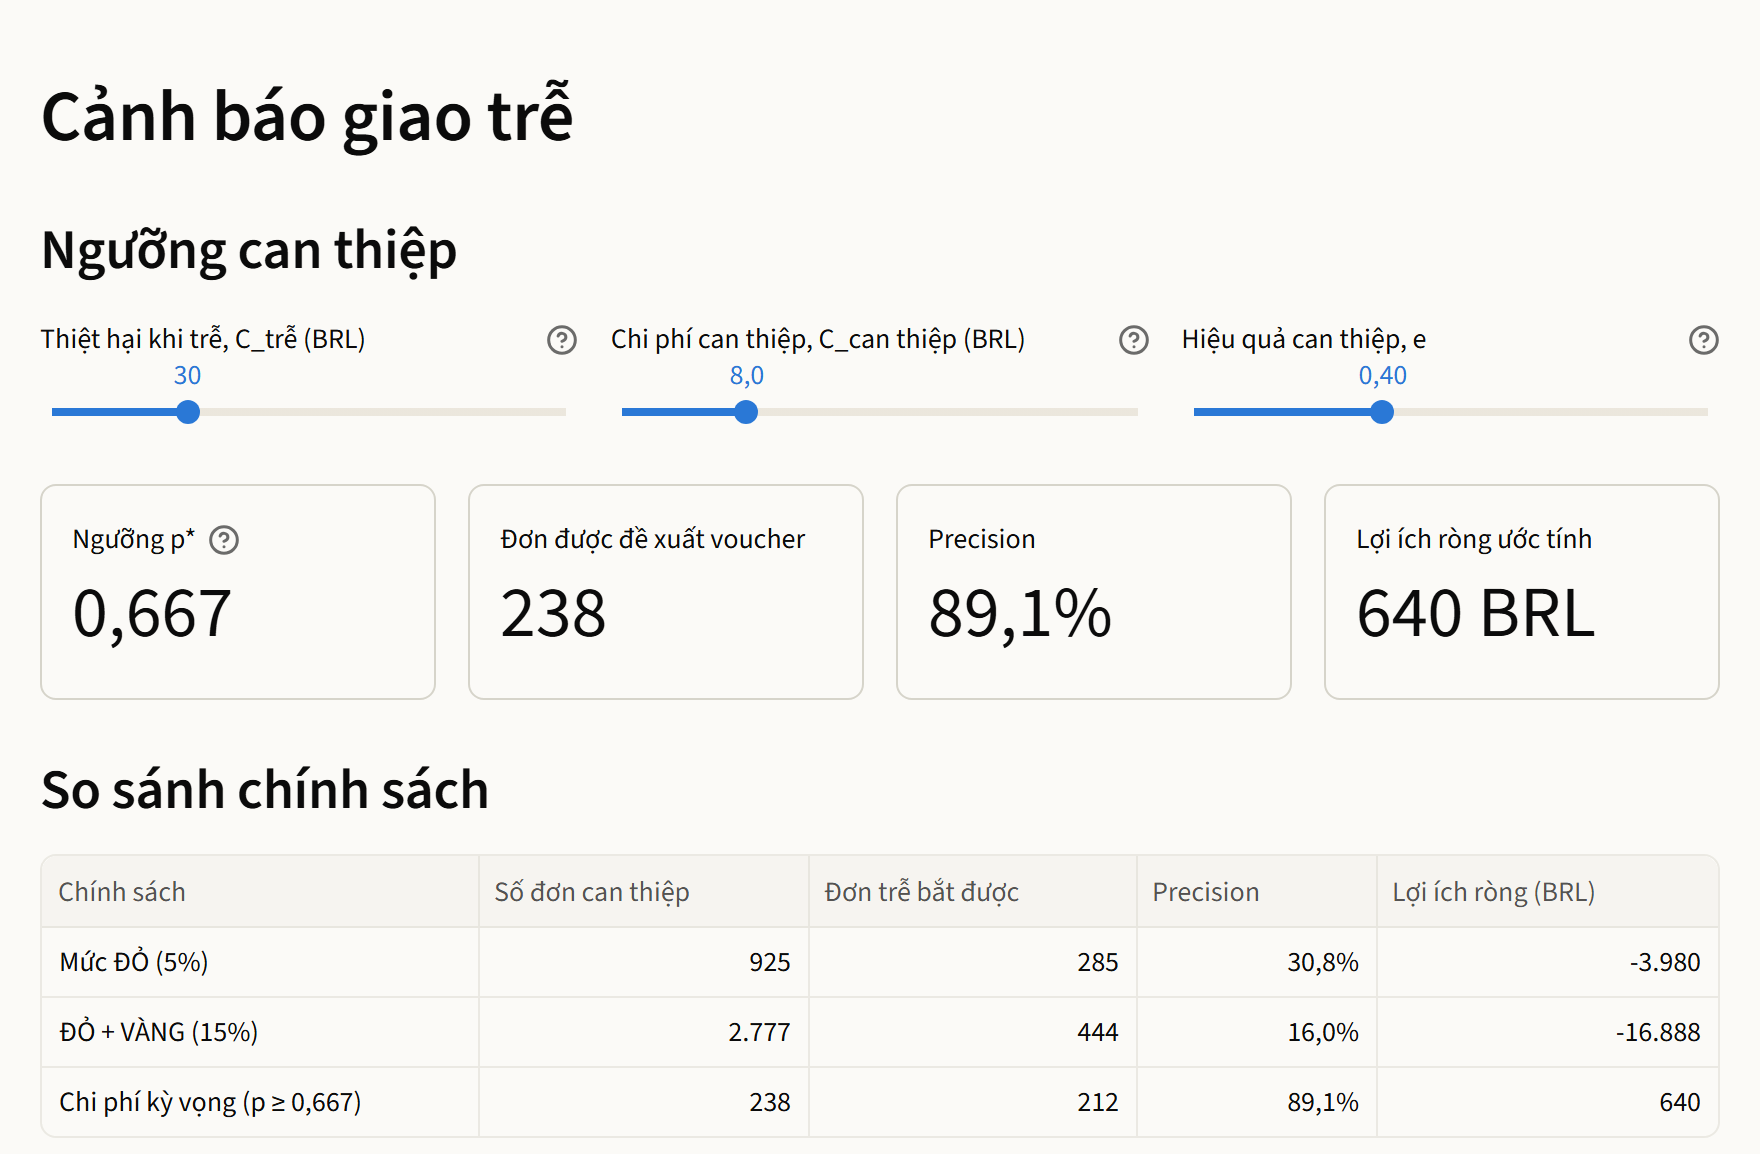
\includegraphics[width=\linewidth]{Pictures/dash-dss-whatif.png}
\caption{Trang Cảnh báo giao trễ, phần what-if: thanh trượt chi phí, ngưỡng $p^{*}$ và so sánh các chính sách}
\label{fig:dashdsswhatif}
\end{figure}

Phần dưới (Hình~\ref{fig:dashdssdanhsach}) là hàng đợi xử lý của một ngày bàn giao, lọc theo mức ĐỎ hoặc VÀNG. Mỗi đơn là một dòng gồm mức rủi ro, mã đơn, xác suất trễ, tối đa ba lý do kèm hành động đề xuất, trạng thái (chờ xử lý, đã duyệt hoặc đã từ chối) và nút thao tác; dòng đếm phía trên cho biết số đơn đã xử lý và còn chờ. Người vận hành nhập tên, có thể ghi chú, rồi bấm ``Duyệt'' hoặc ``Từ chối''; quyết định được ghi vào \code{dss.decision\_log} và đơn đó chuyển sang trạng thái đã duyệt kèm thời điểm, như đơn đầu tiên trên hình. Vì dữ liệu là ba tháng backtest, dòng ``Thực tế'' dưới mỗi đơn cho biết đơn đó sau cùng có trễ hay không; khi triển khai thật, thông tin này chưa có.

\begin{figure}[H]
\centering
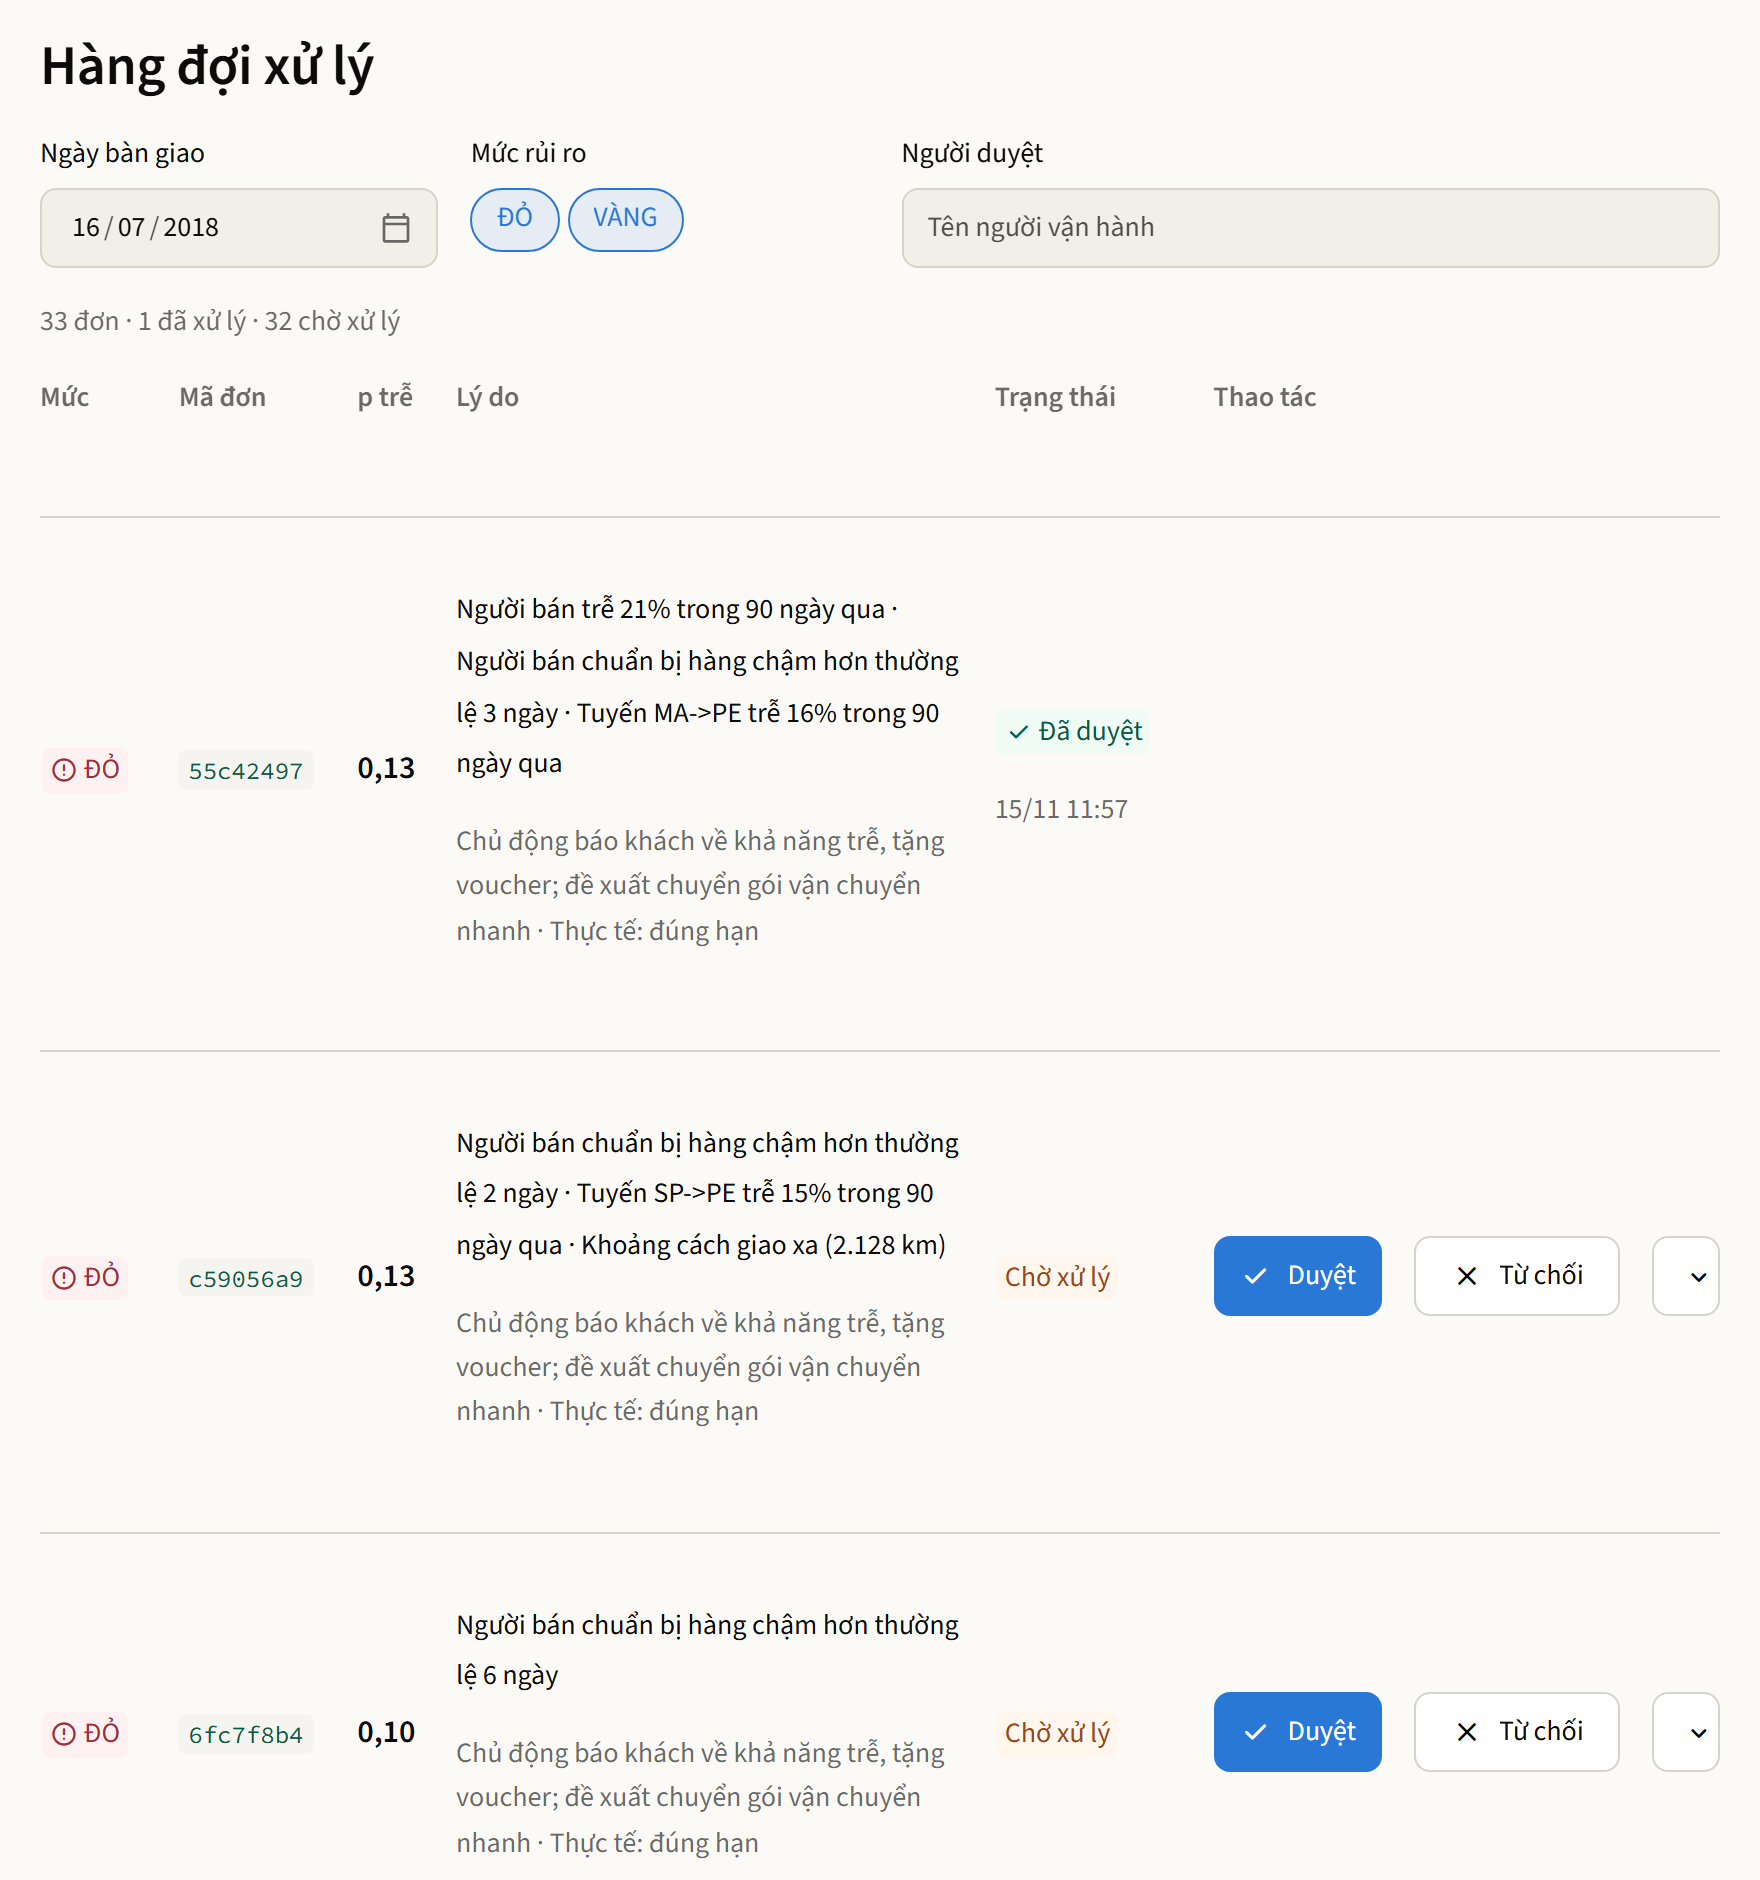
\includegraphics[width=\linewidth]{Pictures/dash-dss-danh-sach.png}
\caption{Trang Cảnh báo giao trễ, hàng đợi xử lý ngày 16/7/2018: lý do cảnh báo, hành động đề xuất, trạng thái và nút duyệt, từ chối}
\label{fig:dashdssdanhsach}
\end{figure}
